\section{Introduction}\label{sec:intro}

The open \texttt{SKILL.\allowbreak{}md} format packages procedural instructions, helper scripts, and reference templates into progressive-disclosure folders loaded on demand by Large Language Model (LLM) coding agents \citep{destefanis2026gitskills, xu2026agentskills}. Yet empirical audits reveal widespread fragility. Mining 3,797,117 public \texttt{SKILL.\allowbreak{}md} files across 282,200 GitHub repositories, \citet{destefanis2026gitskills} note that natural-language skills lack compilers, type checkers, or package verifiers. Across 138,133 public skills, \citet{zhang2026reusable} find 91.8\% contain at least one defect---chiefly bloated instruction bodies and broken metadata---while SkillsBench \citep{li2026skillsbench} shows across 87 tasks and 18 model-harness configurations that curated skills lift pass rates from 33.9\% to 50.5\% (+16.6 percentage points) and focused skills (at most three modules) outperform larger exhaustive bundles. Simultaneously, security studies document high community vulnerability rates \citep{xu2026agentskills, badhe2026skillsecurity}, up to 80\% attack success rate (ASR) on skill-file prompt injections \citep{schmotz2026skillinject}, and semantic supply-chain hijacking \citep{saha2026underhood}.

Research-to-paper authoring stresses all of these weaknesses simultaneously, spanning literature review, experimental execution, visualization, drafting, peer review, and double-blind LaTeX compilation. Existing automated scientific writers---The AI Scientist \citep{lu2024aiscientist}, The AI Scientist-v2 \citep{yamada2025aiscientistv2}, CycleResearcher \citep{weng2024cycleresearcher}, and PaperOrchestra \citep{song2026paperorchestra}---operate as standalone automated pipelines outside interactive coding-agent skill ecosystems. Porting full scientific authoring into interactive coding harnesses exposes four unresolved challenges:

\begin{enumerate}
\def\labelenumi{\arabic{enumi}.}
\tightlist
\item
  \textbf{Context bloat and harness lock-in:} Monolithic playbooks exceed host loader ceilings (e.g., Antigravity's observed 24 KB / 24,000-byte skill limit) and waste prompt context across inactive stages.
\item
  \textbf{Silent provenance and conversion drift:} Without mechanical checks linking manuscript metrics to canonical run logs and citations to saved snapshots, drafting and Markdown-to-LaTeX export silently introduce fabricated decimals, synthetic dry-run leaks, or dropped equations and labels.
\item
  \textbf{Intrinsic self-review bias:} Because LLMs cannot reliably self-correct reasoning without external feedback \citep{huang2024selfcorrect}, same-context self-review misses missing ablations, claim-vs-source contradictions, and prose anonymity leaks.
\item
  \textbf{Scientific supply-chain vectors:} Authoring consumes untrusted abstracts, PDFs, and external conference LaTeX archives---exposing agents to indirect prompt injection \citep{greshake2023indirect}, Zip Slip traversal, LaTeX \texttt{\textbackslash{}write18}/\allowbreak{}\texttt{\textbackslash{}input\{\textbar{}...\}} shell pipes, arbitrary writes, and PDF metadata leaks.
\end{enumerate}

We present \textbf{PaperOEGM} (Paper Orchestra + Elephant-Goldfish Model, adopting the Elephant-Goldfish metaphor of durable workspace memory paired with fresh-context review \citep{google2026egm}), a zero-API-key Agent Skills plugin packaged for Antigravity (live-verified end to end), Claude Code (CLI packaging-validated), and Codex (structurally packaged). PaperOEGM uses zero external LLM API keys and zero third-party Python dependencies for its core verifier (\texttt{po\_\allowbreak{}tools.\allowbreak{}py}), requiring optional \texttt{matplotlib} only for Stage 5 plotting. Its architecture strictly separates \emph{deterministic mechanical verification} from \emph{fresh-context semantic critique} across three layers (Figure~\ref{fig:architecture}): ten budgeted skills (\texttt{\textless{}=\ 12\ KB}, \texttt{disable-model-invocation:\ true}), a standard-library CLI verifier over single-source \texttt{paper\_\allowbreak{}state.\allowbreak{}json}, and five flat single-level read-only critics paired with paranoid LaTeX compilation.

\begin{figure*}[t]
\centering
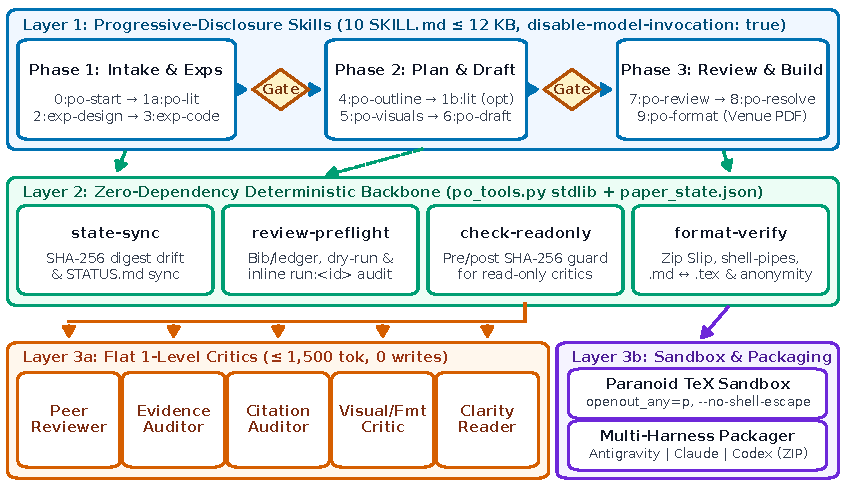
\includegraphics[width=0.88\textwidth]{figures/fig_architecture.pdf}
\caption{PaperOEGM three-layer architecture: progressive-disclosure skills with human checkpoint gates (Layer 1), zero-dependency stdlib verifier backbone (Layer 2), and flat 1-level read-only critics paired with paranoid LaTeX sandboxing and deterministic multi-harness packaging (Layer 3).}
\label{fig:architecture}
\end{figure*}

We make five contributions:

\begin{itemize}
\tightlist
\item
  \textbf{Multi-harness zero-API-key architecture (Section~\ref{sec:method}):} A 10-skill progressive-disclosure graph, single-source \texttt{paper\_\allowbreak{}state.\allowbreak{}json} digest tracker, safe bash experiment contract, flat 1-level read-only critic topology, paranoid TeX wrapper, and deterministic ZIP packager.
\item
  \textbf{PO-FaultBench and deterministic boundaries (Section~\ref{sec:exp-rq1}):} On an author-constructed 120-workspace fault suite (80 faults + 40 hard negative controls per seed, five seeds), \texttt{po\_\allowbreak{}tools.\allowbreak{}py} achieves 100.0\% recall and 0.0\% false-positive rate (FPR) in 108.20 ms/workspace vs.~6.25\% (Compiler-Only) and 87.5\% (No-Inline-Provenance), while recording 0.0\% recall on 20 adversarial evasions/seed---delineating where native sandboxes and semantic critics are mandatory.
\item
  \textbf{Context economics and build determinism (Section~\ref{sec:exp-rq2}):} PaperOEGM reduces median active-stage context by 82.16\% (97.14\% startup index reduction) vs.~monolithic loading, keeps 81.14\% headroom below Antigravity's 24 KB (24,000-byte) ceiling (where public EGM \citep{google2026egm} reaches 24,257 bytes), passes \texttt{claude\ plugin\ validate} with 0 defects, and achieves 100.0\% ZIP SHA-256 parity.
\item
  \textbf{Scalability and paranoid TeX containment (Section~\ref{sec:exp-rq3}):} Across 20--120 citations and 5--30 runs, all four verifier commands run in 266.00--268.55 ms, offload 87.82\%--87.96\% of raw metadata from \texttt{citation\_\allowbreak{}ledger.\allowbreak{}json}, compile three double-blind venues with 0 identity leaks, and block obfuscated shell escapes and parent-directory writes while exposing an upstream TeX Live 2026 \texttt{openin\_\allowbreak{}any=p} no-op regression.
\item
  \textbf{Live hybrid semantic critique (Section~\ref{sec:exp-rq4}):} Across three seeded domain manuscripts (30 planted flaws), deterministic checks catch 100.0\% of mechanical flaws in 91.71 ms but 0.0\% of semantic flaws (50.0\% total), whereas 15 live Antigravity read-only critics recover 100.0\% of semantic flaws with 0.0 clean-control FPs, 0 workspace mutations, and outputs within 1,500 tokens. Limitations are detailed in Section~\ref{sec:limitations}.
\end{itemize}
